\chapter{Barrier Option Pricing with Monte Carlo}

\begin{figure}[h]
	\centering
	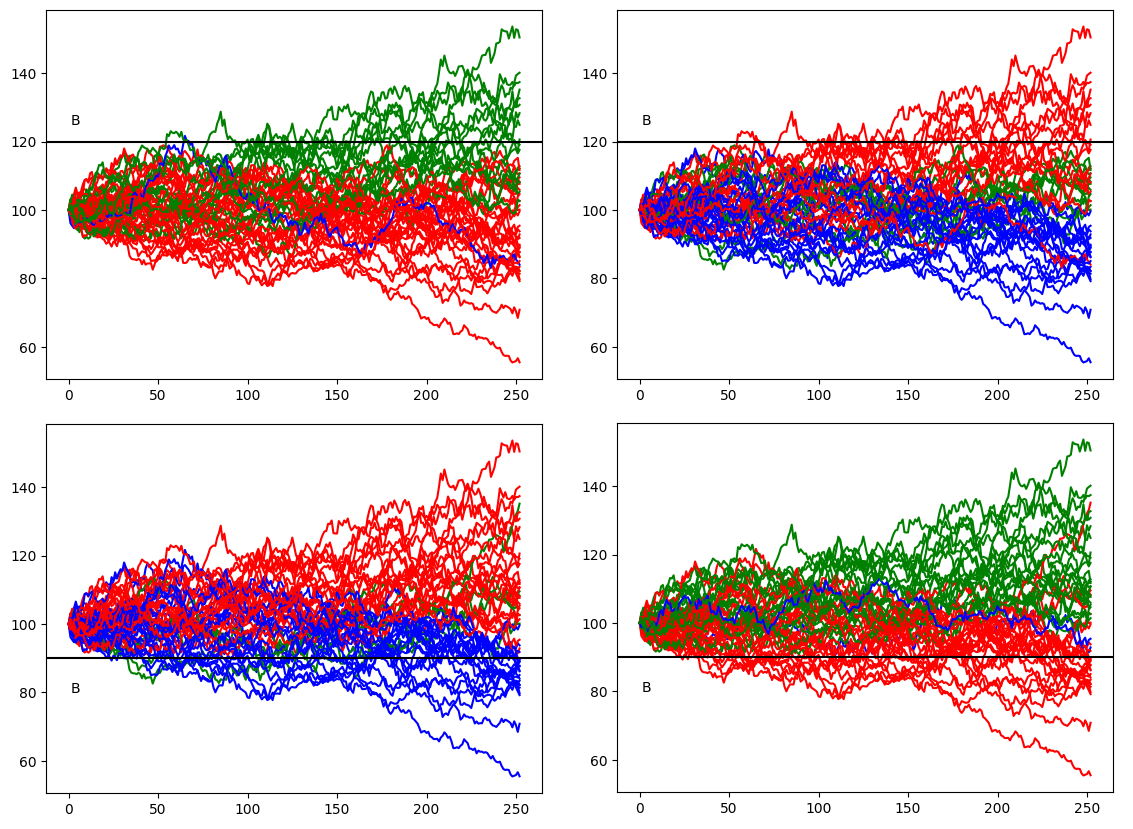
\includegraphics[width=.65\linewidth]{content/images/monte_carlo_paths.png}
	\caption{Simulated Paths Barrier Option Prices using Monte Carlo}
	\label{fig:monte_carlo_paths}
\end{figure}
Suppose the asset price follows a Geometric Brownian Motion (GBM):
\begin{equation}\label{eq:GBM}
	dS_t=rS_tdt+\sigma S_tdW_t
\end{equation}
Where $S_t$ is the asset price at time $t$, $r$ is the risk-free interest rate, $\sigma$ is the volatility of the asset, and $dW_t$ is the increment of a Wiener process. With this process in mind, we can discretize time by dividing the total time into smaller length intervals $\Delta t=T/N.$ Afterwards, we simulate the asset price paths by generating a random standard normal variable $Z$ and using the random variable to update the asset price with the discretized GBM. 
\begin{equation}
	S_{t+\Delta t}=S_t\times\exp\left(\left(r-\frac{\sigma^2}{2}\right)\Delta t+\sigma\sqrt{\Delta t}\times 2\right)
\end{equation}

The Monte Carlo simulation is a tool that we can implement to analyze models like GBM. Monte Carlo is a computational algorithm that uses repeated random sampling to obtain numerical results. It is used to predict the behavior of complex systems that are difficult to model analytically (while European Barrier options have an analytical solution, we will still incorporate Monte Carlo). In the context of GBM, Monte Carlo simulations are used to simulate many possible paths of stock prices over time under the assumptions of GBM. This allows for exploring statistical outcomes and quantifying risk in a financial context, where analytical solutions may be challenging to reproduce. 

Figure (\ref{fig:monte_carlo_paths}) shows the simulated Monte Carlo paths for all of the barrier call options: up-and-in (top left), up-and-out (top right), down-and-in (bottom left), and down-and-out (bottom right). We assume the $S=100, K=100, T=1,r=5\%,\text{ and } \sigma=20\%$. We use a barrier, $B$, of 120 for the up-in/up-out options and 90 for the down-in/down-out options. We highlight the path's different colors based on the outcome at the expiration date. 

Take the up-and-in (top-left) barrier option, for example. If the simulated stock path breaches the barrier and stays above the strike price, $K$, we highlight the path as green. If the stock breaches the barrier but ends below the strike price, we highlight the path as blue (the option becomes exercisable but expires out-of-the-money). All other paths will be highlighted in red if the simulated paths never breach the barrier level. Other simulations utilize the same criteria for their path directions based on the characteristics of the option. 

We have only used 100 simulations, as it is easier to display the different outcomes. Regardless, we can see that we can consistently arrive at an option price that mirrors the analytical model simply by averaging the outcomes where $K<S<B$, as we are working with an up-and-out.
\newpage
\section{Monte Carlo Simulation}

Table (\ref{tab:MC_barrer}) shows the comparison between the Black-Scholes analytical price and the Monte Carlo simulations for the up-and-out call options. We have chosen options with different Barrier values as well as varying stock values.

\begin{center}
	\begin{table}[H]
		\begin{tabular}{ | m{4em} | m{1.4cm}| m{1.4cm} | m{1.4cm}| m{1.4cm} | m{1.37cm} | m{1.4cm} | m{1.4cm} | m{1.4cm} | m{1.45cm} |} 
			\hline
			& Price & $\text{MC}_{100}$ & $\text{err}_{100}$ & $\text{MC}_{1000}$ & $\text{err}_{1000}$ & $\text{MC}_{5000}$ & $\text{err}_{5000}$ & $\text{MC}_{10000}$ & $\text{err}_{10000}$  \\ 
			\hline
			$S_0=90$ $B=120$ & 1.2925 (7.3823) & 1.8113 (8.0324)  & -0.5188 (-0.6524) & 1.4851 (7.5403) & -0.1926 (-0.1603) & 1.3249 (7.4427) & -0.0324 (-0.0627) & 1.3525 (7.3643) & -0.06 (0.0157) \\ 
			\hline
			$S_0=90$ $B=130$ & 2.9799 (7.5049) & 3.2746 (6.7301) & -0.2947 (0.7748) & 3.0758 (7.9160) & -0.0960 (-0.4111) &  3.0351 (7.4177) & -0.0552 (0.0872) & 2.9991 (7.4826) & -0.0192 (0.0222) \\ 
			\hline
			$S_0=100$ $B=120$ & 1.1789 (3.5932) & 1.5790 (4.0435) & -0.4001 (-0.4503) & 1.0808 (3.9701)  & 0.0981 (-0.3763) & 1.2127 (3.6234) & -0.0338 (-0.0302) & 1.2060 (3.5990) & -0.0271 (-0.0058) \\ 
			\hline
			$S_0=100$ $B=130$ & 3.5369 (3.7432) & 4.6782 (4.4019)  & -1.1413 (-0.6587) & 3.2785 (3.8816) & 0.2584 (-0.1384) & 3.4410 (3.7508) & 0.0959 (-0.0076) & 3.5303 (3.7498)  & 0.0066 (-0.0066)\\ 
			\hline 
			$S_0=110$ $B=120$ & 0.6264 (1.3437) & 0.7961 (1.5428) & -0.1697 (-0.1991) & 0.7819 (1.2988) & -0.1555 (0.0449) & 0.6422 (1.3553) & -0.0159 (-0.0116) & 0.6551 (1.3396) & -0.0362 (0.0041) \\
			\hline
			$S_0=110$ $B=130$ & 2.9014 (1.6735) & 2.4881 (1.5780)  & 0.4133 (0.0955) & 3.1815 (1.8227) & -0.2801 (-0.1492) & 2.9130 (1.7561) & -0.0116 (-0.0826) & 2.9700 (1.6167) & -0.0686 (0.0568)\\
			\hline
			$S_0=110$ $B=250$ & 13.2660 (3.7534) & 13.4717 (4.6529)  & -0.2057 (-0.8995) & 13.0827 (4.2545) & 0.1833 (-0.5011) & 13.1939 (3.5797) & 0.0721 (0.1737) & 13.2129 (3.7706) & 0.0531 (-0.0172)\\
			\hline
		\end{tabular}
		\caption{MC Up-and-out call with $q=0\%,r=10\%, T=1,\sigma=20\%,K=100$}
		\label{tab:MC_barrer}
	\end{table}
\end{center}

These results will be compared with those obtained through alternative variations of Monte Carlo methods. We've used simulations $n=100$, the same number as in Figure (\ref{fig:monte_carlo_paths}), but we also use simulations where $n=1000,5000,\text{ and }10000$, as well. The errors listed in the tables represent the price deviation from the analytical values. The values in the parenthesis denote the outcome for puts, while the values without parenthesis denote the values for calls. As we can see, the Monte Carlo price gets closer to the analytical solution for $n=5000$. With the table, we confirm one main aspect of Monte Carlo theory: increasing the number of simulations leads to an improved accuracy for the computation. 

We have also used a simulation with an arbitrarily high barrier of 250 and the results simulate what we can expect from the Monte Carlo method, as well as the analytical method. When the barrier is very far away from the underlying price, the option value will mirror the Black-Scholes price.
